\documentclass[aspectratio=169]{beamer}
\usepackage{graphicx}
\usepackage{listings}
\usepackage{xcolor}
\usepackage{amsmath}
% SVGs pre-converted to PDF via inkscape

% Custom footline with slide numbers in bottom left
\setbeamertemplate{footline}{
  \hspace{1em}%
  \usebeamercolor[fg]{page number in head/foot}%
  \usebeamerfont{page number in head/foot}%
  \insertframenumber\,/\,\inserttotalframenumber%
  \vskip2pt%
}

\beamertemplatenavigationsymbolsempty

% Code listing style
\lstset{
  basicstyle=\ttfamily\tiny,
  keywordstyle=\color{blue}\bfseries,
  commentstyle=\color{gray}\itshape,
  stringstyle=\color{orange},
  showstringspaces=false,
  breaklines=true,
  frame=single,
  backgroundcolor=\color{gray!10},
  rulecolor=\color{gray!50},
  xleftmargin=2pt,
  xrightmargin=2pt,
  aboveskip=4pt,
  belowskip=4pt,
}

\title{FRIDA Design Review}
\author{Kennedy Caisley}
\date{Wednesday, 28 January 2026}

\begin{document}

\begin{frame}
  \titlepage
\end{frame}

%% ============================================================
%% FRIDA Chip Overview
%% ============================================================
\begin{frame}
  \frametitle{FRIDA Chip Overview}
  \begin{columns}
    \begin{column}{0.65\textwidth}
      \begin{center}
        \includegraphics[width=\linewidth,height=0.85\textheight,keepaspectratio]{images/adc_basic.pdf}
      \end{center}
    \end{column}
    \begin{column}{0.35\textwidth}
      \begin{center}
        \includegraphics[width=\linewidth,height=0.85\textheight,keepaspectratio]{images/frida_65A.png}
      \end{center}
    \end{column}
  \end{columns}
\end{frame}

%% ============================================================
%% Floorplan Overview (ASCII)
%% ============================================================
\begin{frame}[fragile]
  \frametitle{Sketch of ADC Floorplan}
  \centering
  \begin{lstlisting}[basicstyle=\ttfamily\fontsize{4}{5}\selectfont,frame=none,backgroundcolor=\color{white}]
            Logic and Macro Placement (FEOL-M3)           Power Domain Placement (M3-M4)              Capacitor DAC Arrays (M5-M6)
            -----------------------------------           ------------------------------              ----------------------------

     +-    +----------------------------------+        +----------------------------------+        +---------------+  +---------------+
2 Tr |     |         Cap Drivers (diff)       |        |         vdd_dac & vss_dac        |        |    (pins)     |  |    (pins)     |
     +-    +----------------------------------+        +----------------------------------+        |               |  |               |
     +-    +---+ +------++------++------+ +---+             +------------------------+             |               |  |               |
     |     |   | |      ||      ||      | |   |             |                        |             |               |  |               |
5 Tr |     |   | | SW N || Comp || SW P | |   |             |     vdd_a & vss_a      |             |               |  |               |
     |     |   | |      ||      ||      | |   |             |                        |             |               |  |               |
     +-    |   | +------++------++------+ |   |             +------------------------+             |               |  |               |
     +-    |   +---------------------------   |        +----------------------------------+        |               |  |               |
     |     |                                  |        |                                  |        |               |  |               |
     |     |                                  |        |                                  |        |               |  |               |
     |     |                                  |        |                                  |        |               |  |               |
     |     |                                  |        |                                  |        |  P Cap Array  |  |  N Cap Array  |
     |     |                                  |        |                                  |        |               |  |               |
8 Tr |     |        SA Logic, Clk Gate,       |        |          vdd_d & vss_d           |        |               |  |               |
     |     |           & Samp Driver          |        |                                  |        |               |  |               |
     |     |                                  |        |                                  |        |               |  |               |
     |     |                                  |        |                                  |        |               |  |               |
     |     |                                  |        |                                  |        |               |  |               |
     |     |                                  |        |                                  |        |               |  |               |
     +-    +----------------------------------+        +----------------------------------+        |               |  |               |
     +-    +----------------------------------+        +----------------------------------+        |               |  |               |
2 Tr |     |        Cap Drivers (main)        |        |        vref_p  & vref_n          |        |    (pins)     |  |    (pins)     |
     +-    +----------------------------------+        +----------------------------------+        +---------------+  +---------------+
  \end{lstlisting}
\end{frame}

%% ============================================================
%% ADC Digital Netlist
%% ============================================================
\begin{frame}
  \frametitle{ADC Digital Block Netlist}
  \begin{columns}
    \begin{column}{0.35\textwidth}
      \begin{itemize}
        \item \textbf{salogic}: SAR sequencing FSM
        \item \textbf{clkgate}: Clock gating for power
        \item \textbf{sampdriver\_p/n}: Sampling switch drivers
        \item Symmetric P/N halves for differential operation
        \item salogic and clkgate shared between halves
      \end{itemize}
    \end{column}
    \begin{column}{0.65\textwidth}
      \begin{center}
        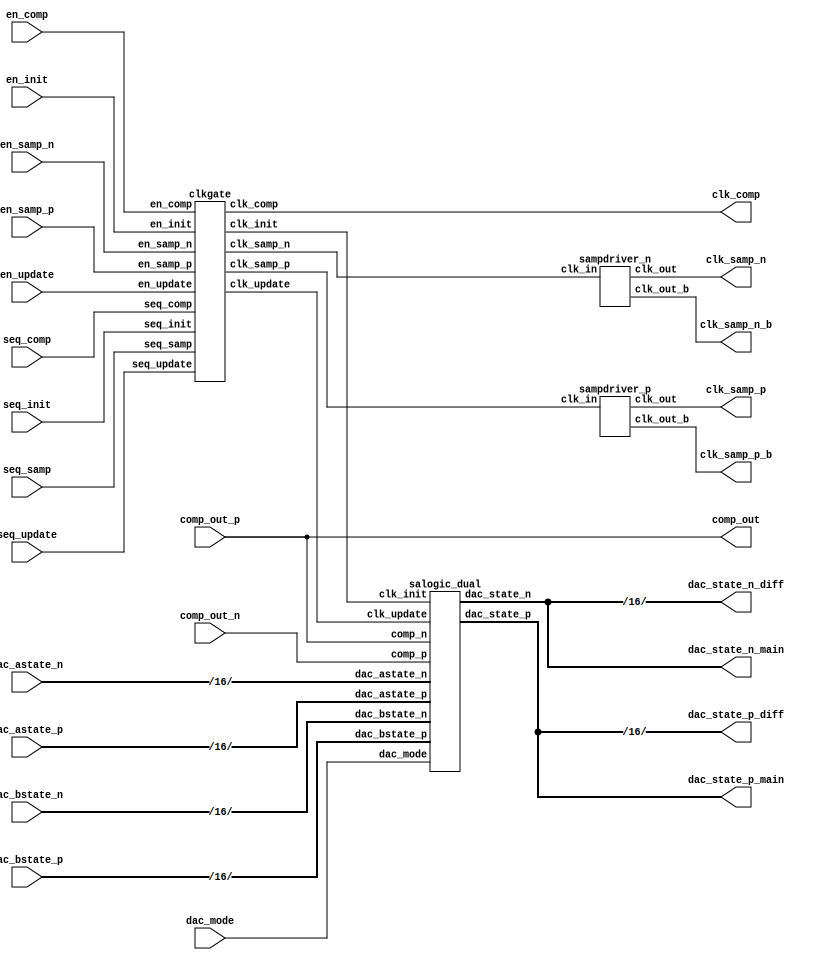
\includegraphics[width=\linewidth,height=0.85\textheight,keepaspectratio]{images/adc_digital_netlistsvg.pdf}
      \end{center}
    \end{column}
  \end{columns}
\end{frame}

%% ============================================================
%% OpenROAD Flow Scripts Overview
%% ============================================================
\begin{frame}
  \frametitle{OpenROAD Flow Scripts (ORFS)}
  \begin{columns}
    \begin{column}{0.5\textwidth}
      \begin{itemize}
        \item \textbf{Yosys}: RTL synthesis
          \begin{itemize}
            \item Verilog parsing and elaboration
            \item Logic optimization (ABC)
            \item Technology mapping to standard cells
          \end{itemize}
        \item \textbf{OpenROAD}: Physical design
          \begin{itemize}
            \item Floorplanning and PDN
            \item Placement (global + detailed)
            \item Clock tree synthesis
            \item Routing (global + detailed)
            \item Timing analysis (OpenSTA)
          \end{itemize}
        \item \textbf{KLayout}: Final verification
          \begin{itemize}
            \item DRC and LVS checks
            \item GDS export
          \end{itemize}
      \end{itemize}
    \end{column}
    \begin{column}{0.5\textwidth}
      \begin{center}
        \includegraphics[width=\linewidth,height=0.85\textheight,keepaspectratio]{images/orfs.png}
      \end{center}
    \end{column}
  \end{columns}
\end{frame}

%% ============================================================
%% Yosys: Step 1 - Synthesis
%% ============================================================
\begin{frame}[fragile]
  \frametitle{Yosys: Step 1 - RTL Synthesis}
  \begin{columns}
    \begin{column}{0.5\textwidth}
      \textbf{Input Files}
      \begin{itemize}
        \item adc\_digital.v (top module)
        \item clkgate.v, salogic.v, sampdriver.v
        \item cells\_tsmc65.v (cell wrappers)
      \end{itemize}
      \vspace{1em}
      \textbf{Synthesis Statistics}
      \begin{itemize}
        \item Total cells: 350
        \item Total area: 893.88 $\mu$m$^2$
        \item Sequential elements: 49\% of area
        \item 48 flip-flops (DFQD1, EDFD2)
        \item 5 clock gates (CKLNQD1LVT)
      \end{itemize}
    \end{column}
    \begin{column}{0.5\textwidth}
      \textbf{Technology Mapping (ABC)}
      \begin{lstlisting}[basicstyle=\ttfamily\scriptsize]
Module         Cells    Area
---------------------------------
adc_digital       38    54.36
  clkgate          6    33.48
  salogic        302   798.84
  sampdriver       2     3.60
---------------------------------
Total            350   893.88
      \end{lstlisting}
      \vspace{0.5em}
      \textbf{Key Cell Types}
      \begin{lstlisting}[basicstyle=\ttfamily\scriptsize]
EDFD2LVT (edge DFF)     32   334.08
DFQD1LVT (DFF)          16   109.44
NR2D0LVT (NOR2)         93   133.92
BUFFD0LVT (buffer)      69    99.36
CKLNQD1LVT (clkgate)     5    32.40
      \end{lstlisting}
    \end{column}
  \end{columns}
\end{frame}

%% ============================================================
%% OpenROAD Step 2.1 Floorplan
%% ============================================================
\begin{frame}[fragile]
  \frametitle{OpenROAD Step 2.1: Floorplan}
  \begin{columns}
    \begin{column}{0.45\textwidth}
      \begin{center}
        \includegraphics[width=\linewidth,height=0.85\textheight,keepaspectratio]{images/2_0_floorplan.png}
      \end{center}
    \end{column}
    \begin{column}{0.55\textwidth}
      \begin{itemize}
        \item Die and core area: 60$\mu$m $\times$ 49$\mu$m
        \item Row height: 2.8$\mu$m (17 rows)
        \item Blockages reserve space for analog macros
        \item I/O pin and routing grid (0.2$\mu$m pitch)
      \end{itemize}
      \vspace{1em}
      \textbf{config.mk}
      \begin{lstlisting}[language=make]
export DIE_AREA = 0 0 60 49
export CORE_AREA = 0 0 60 49
export CREATE_BLOCKAGES = .../create_blockages.tcl
      \end{lstlisting}
      \textbf{create\_blockages.tcl}
      \begin{lstlisting}[language=tcl]
# Reserve area for comparator
create_blockage -region {17.5 27.0 42.5 49}
# Reserve areas for sampling switches
create_blockage -region {12.5 42.6 21 49}
create_blockage -region {39 42.6 47.5 49}
      \end{lstlisting}
    \end{column}
  \end{columns}
\end{frame}

%% ============================================================
%% OpenROAD Step 2.2 Floorplan with PDN
%% ============================================================
\begin{frame}[fragile]
  \frametitle{OpenROAD Step 2.2: Power Distribution Network}
  \begin{columns}
    \begin{column}{0.45\textwidth}
      \begin{center}
        \includegraphics[width=\linewidth,height=0.85\textheight,keepaspectratio]{images/2_4_floorplan_pdn.png}
      \end{center}
    \end{column}
    \begin{column}{0.55\textwidth}
      \begin{itemize}
        \item M4 vertical stripes at edges for vdd\_d/vss\_d
        \item M1 horizontal stripes follow cell rows
        \item M1-M4 connections for power delivery
      \end{itemize}
      \vspace{1em}
      \textbf{pdn.tcl}
      \begin{lstlisting}[language=tcl]
add_global_connection -net {vdd_d} \
  -inst_pattern {.*} -pin_pattern VDD -power
add_global_connection -net {vss_d} \
  -inst_pattern {.*} -pin_pattern VSS -ground

define_pdn_grid -name "Core" -pins {M4}

add_pdn_stripe -grid "Core" -layer M4 \
  -width 0.4 -offset 1.3 -nets {vdd_d}
add_pdn_stripe -grid "Core" -layer M4 \
  -width 0.4 -offset 2.1 -nets {vss_d}

add_pdn_stripe -grid "Core" -layer M1 \
  -followpins -width 0.33
add_pdn_connect -grid "Core" -layers {M1 M4}
      \end{lstlisting}
    \end{column}
  \end{columns}
\end{frame}

%% ============================================================
%% OpenROAD Step 3.1 Global Placement (Skip IO)
%% ============================================================
\begin{frame}[fragile]
  \frametitle{OpenROAD Step 3.1: Global Placement}
  \begin{columns}
    \begin{column}{0.45\textwidth}
      \begin{center}
        \includegraphics[width=\linewidth,height=0.85\textheight,keepaspectratio]{images/3_1_place_gp_skip_io.png}
      \end{center}
    \end{column}
    \begin{column}{0.55\textwidth}
      \begin{itemize}
        \item Initial cell location doesn't consider I/O
        \item Instead routability-driven placement
        \item 60\% target placement density
        \item Placement avoids blockages
        \
      \end{itemize}
      \vspace{1em}
      \textbf{config.mk}
      \begin{lstlisting}[language=make]
# Standard cell placement density
export PLACE_DENSITY = 0.50

# I/O pin layers
export IO_PLACER_H = M3
export IO_PLACER_V = M2
      \end{lstlisting}
    \end{column}
  \end{columns}
\end{frame}

%% ============================================================
%% OpenROAD Step 3.2 Global Placement
%% ============================================================
\begin{frame}[fragile]
  \frametitle{OpenROAD Step 3.2: Global Placement (I/O Aware)}
  \begin{columns}
    \begin{column}{0.45\textwidth}
      \begin{center}
        \includegraphics[width=\linewidth,height=0.85\textheight,keepaspectratio]{images/3_3_place_gp.png}
      \end{center}
    \end{column}
    \begin{column}{0.55\textwidth}
      \begin{itemize}
        \item Cells migrated toward connected IO pins
        \item 445 movable cells, 457 total instances
        \item Timing-driven with Nesterov solver
        \item 335 iterations to converge
      \end{itemize}
      \vspace{0.5em}
      \begin{center}
      \small
      \begin{tabular}{l|r}
        \hline
        \textbf{Metric} & \textbf{Value} \\
        \hline
        Core area & 2916 $\mu$m$^2$ \\
        Cell area & 1102 $\mu$m$^2$ \\
        Utilization & 49\% \\
        Final HPWL & 5125 $\mu$m \\
        Worst slack & 4.49 ns \\
        fmax achievable & 1975 MHz \\
        \hline
      \end{tabular}
      \end{center}
    \end{column}
  \end{columns}
\end{frame}

%% ============================================================
%% OpenROAD Step 3.3 Detailed Placement
%% ============================================================
\begin{frame}[fragile]
  \frametitle{OpenROAD Step 3.3: Detailed Placement}
  \begin{columns}
    \begin{column}{0.45\textwidth}
      \begin{center}
        \includegraphics[width=\linewidth,height=0.85\textheight,keepaspectratio]{images/3_5_place_dp.png}
      \end{center}
    \end{column}
    \begin{column}{0.55\textwidth}
      \begin{itemize}
        \item 424 cells legalized to row sites
        \item Legalization adds 4\% HPWL
        \item Optimization recovers 9.8\% HPWL
      \end{itemize}
      \vspace{0.5em}
      \textbf{Optimization Passes}
      \begin{lstlisting}[basicstyle=\ttfamily\scriptsize]
Independent set matching   0.35%
Global swaps               2.36%
Vertical swaps             0.34%
Reordering                 0.96%
Random improvement         3.09%
Cell flipping              3.10%
      \end{lstlisting}
      \vspace{0.3em}
      \small
      \begin{tabular}{l|r}
        \hline
        \textbf{Metric} & \textbf{Value} \\
        \hline
        Final HPWL & 4796 $\mu$m \\
        Final area & 1102 $\mu$m$^2$ \\
        Utilization & 38\% \\
        \hline
      \end{tabular}
    \end{column}
  \end{columns}
\end{frame}

%% ============================================================
%% OpenROAD Step 4.1 Clock Tree Synthesis
%% ============================================================
\begin{frame}[fragile]
  \frametitle{OpenROAD Step 4.1: Clock Tree Synthesis}
  \begin{columns}
    \begin{column}{0.45\textwidth}
      \begin{center}
        \includegraphics[width=\linewidth,height=0.85\textheight,keepaspectratio]{images/4_1_cts.png}
      \end{center}
    \end{column}
    \begin{column}{0.55\textwidth}
      \begin{itemize}
        \item System clock: 10 MHz (100ns period)
        \item Samp/comp clock: 200 MHz (5ns period)
        \item 50ps clock uncertainty
        \item Balanced tree for minimal skew
      \end{itemize}
      \vspace{1em}
      \textbf{constraint.sdc}
      \begin{lstlisting}[language=tcl]
current_design adc_digital

# Create clock for sequencing (200 MHz)
create_clock -name seq_update \
  -period 5 [get_ports seq_update]

# Set clock uncertainties
set_clock_uncertainty 0.05 [all_clocks]
      \end{lstlisting}
    \end{column}
  \end{columns}
\end{frame}

%% ============================================================
%% OpenROAD Step 4.1 Clock Tree Views
%% ============================================================
\begin{frame}
  \frametitle{OpenROAD Step 4.1: Clock Tree Views}
  \begin{columns}
    \begin{column}{0.5\textwidth}
      \begin{center}
        \includegraphics[width=\linewidth,height=0.85\textheight,keepaspectratio]{images/4_1_cts_alt.png}
      \end{center}
    \end{column}
    \begin{column}{0.5\textwidth}
      \begin{center}
        \includegraphics[width=0.9\linewidth,height=0.35\textheight,keepaspectratio]{images/4_1_treeview.png}
      \end{center}
      \vspace{0.3em}
      \small
      \textbf{CTS Results:}
      \begin{itemize}
        \item 31 BUFFD2LVT cells across 4 clock paths
        \item Domains unsynchronized within ADC (relies on upstream sequencer)
        \item Clock power: 41\% of total
        \item Setup skew: 0.07 ns
      \end{itemize}
    \end{column}
  \end{columns}
\end{frame}

%% ============================================================
%% OpenROAD Step 5.1 Global Routing
%% ============================================================
\begin{frame}[fragile]
  \frametitle{OpenROAD Step 5.1: Global Routing}
  \begin{columns}
    \begin{column}{0.45\textwidth}
      \begin{center}
        \includegraphics[width=\linewidth,height=0.85\textheight,keepaspectratio]{images/5_1_routeguides_global.png}
      \end{center}
    \end{column}
    \begin{column}{0.55\textwidth}
      \begin{itemize}
        \item Route guides shown for global routing
        \item M2-M3 routing layers only
        \item Routing obstructions for analog areas
      \end{itemize}
      \vspace{1em}
      \textbf{config.mk}
      \begin{lstlisting}[language=make]
export MIN_ROUTING_LAYER = M2
export MAX_ROUTING_LAYER = M3
export PRE_GLOBAL_ROUTE_TCL = \
  .../routing_blockages.tcl
      \end{lstlisting}
      \textbf{routing\_blockages.tcl}
      \begin{lstlisting}[language=tcl]
# Create obstructions on M1-M4 for analog
odb::dbObstruction_create $block $layer_M1 \
  $comp_llx $comp_lly $comp_urx $comp_ury
odb::dbObstruction_create $block $layer_M2 \
  $comp_llx $comp_lly $comp_urx $comp_ury
      \end{lstlisting}
    \end{column}
  \end{columns}
\end{frame}

%% ============================================================
%% OpenROAD Step 5.2 Detailed Routing
%% ============================================================
\begin{frame}[fragile]
  \frametitle{OpenROAD Step 5.2: Detailed Routing}
  \begin{columns}
    \begin{column}{0.45\textwidth}
      \begin{center}
        \includegraphics[width=\linewidth,height=0.85\textheight,keepaspectratio]{images/5_2_route.png}
      \end{center}
    \end{column}
    \begin{column}{0.55\textwidth}
      \begin{itemize}
        \item Final metal routing on M2/M3
        \item All signals routed to I/O pins
        \item DRC-clean routing around blockages
        \item \textbf{Issue:} Multicut vias on large devices
      \end{itemize}
      \vspace{0.5em}
      \begin{center}
      \small
      \begin{tabular}{l|r}
        \hline
        \textbf{Metric} & \textbf{Value} \\
        \hline
        Nets routed & 506 \\
        Total wire length & 5717 $\mu$m \\
        M2 wire length & 3183 $\mu$m \\
        M3 wire length & 2625 $\mu$m \\
        Total vias & 2058 \\
        Clock skew & 0.07 ns \\
        Worst slack & 4.37 ns \\
        \hline
      \end{tabular}
      \end{center}
    \end{column}
  \end{columns}
\end{frame}

%% ============================================================
%% OpenROAD Step 5.3 Fill Cells
%% ============================================================
\begin{frame}[fragile]
  \frametitle{OpenROAD Step 5.3: Fill Cells}
  \begin{columns}
    \begin{column}{0.45\textwidth}
      \begin{center}
        \includegraphics[width=\linewidth,height=0.85\textheight,keepaspectratio]{images/5_3_fillcell.png}
      \end{center}
    \end{column}
    \begin{column}{0.55\textwidth}
      \begin{itemize}
        \item Decap fill cells added (FEOL)
        \item Metal fill disabled (BEOL)
        \item Fills gaps in standard cell rows
      \end{itemize}
      \vspace{1em}
      \textbf{config.mk}
      \begin{lstlisting}[language=make]
# Only disables metal fill
# FILL_CELLS in routing step still
# adds FEOL decap fill cells
export USE_FILL = 0
      \end{lstlisting}
    \end{column}
  \end{columns}
\end{frame}

%% ============================================================
%% OpenROAD Step 6.1 Heat Maps
%% ============================================================
\begin{frame}
  \frametitle{OpenROAD Step 6.1: Heat Maps}
  \begin{columns}
    \begin{column}{0.45\textwidth}
      \begin{center}
        \includegraphics[width=\linewidth,height=0.85\textheight,keepaspectratio]{images/6_2_thermal.png}
      \end{center}
    \end{column}
    \begin{column}{0.55\textwidth}
      \begin{flushleft}
        \includegraphics[width=0.6\linewidth,height=0.25\textheight,keepaspectratio]{images/power.png}
      \end{flushleft}
      \vspace{0.5em}
      \begin{itemize}
        \item Spatial visualizations for IR drop, thermal dissipation, placement density, pin density, and power consumption
        \item DRC and antenna violation views for debugging
      \end{itemize}
    \end{column}
  \end{columns}
\end{frame}

%% ============================================================
%% OpenROAD GUI
%% ============================================================
\begin{frame}
  \frametitle{OpenROAD GUI}
  \begin{itemize}
    \item Interactive GUI, net tracing, hierarchical cell grouping, timing reports, DRC viewer, heatmaps
  \end{itemize}
  \begin{center}
    \includegraphics[width=\linewidth,height=0.78\textheight,keepaspectratio]{images/openroad_gui.png}
  \end{center}
\end{frame}

%% ============================================================
%% ADC Digital Layout
%% ============================================================
\begin{frame}
  \frametitle{ADC Digital Block Layout}
  \begin{columns}
    \begin{column}{0.55\textwidth}
      \begin{center}
        \includegraphics[width=\linewidth,height=0.85\textheight,keepaspectratio]{images/frida_adc_dgital.png}
      \end{center}
    \end{column}
    \begin{column}{0.45\textwidth}
      \begin{center}
      \small
      \begin{tabular}{l|r}
        \hline
        \textbf{Metric} & \textbf{Value} \\
        \hline
        Dimensions & 60$\times$49 $\mu$m \\
        Cell count & 350 \\
        Area & 894 $\mu$m$^2$ \\
        Flip-flops & 48 \\
        Clock gates & 5 \\
        Wire length & 5717 $\mu$m \\
        Vias & 2058 \\
        Power & 18 $\mu$W \\
        \hline
      \end{tabular}
      \end{center}
    \end{column}
  \end{columns}
\end{frame}

%% ============================================================
%% ADC Top Assembly
%% ============================================================
\begin{frame}
  \frametitle{ADC Top-Level Assembly}
  \begin{center}
    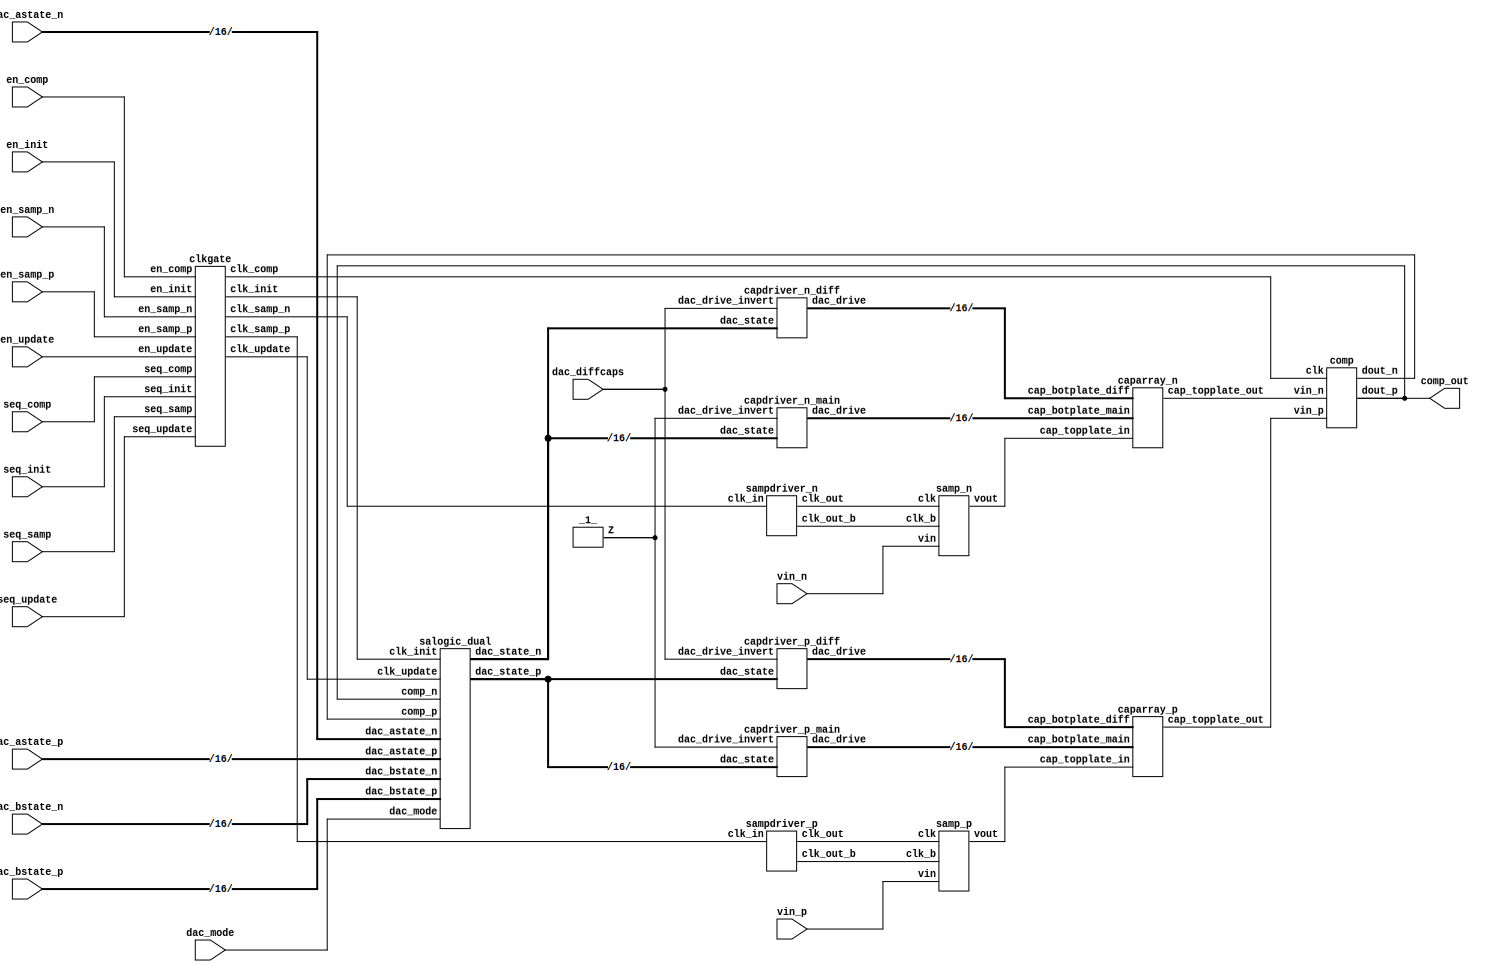
\includegraphics[width=\linewidth,height=0.75\textheight,keepaspectratio]{images/adc_top_netlistsvg.pdf}
  \end{center}
  \begin{itemize}
    \item ADC assembled using hierarchical Verilog as well, with protected routing for sensitive analog nets
  \end{itemize}
\end{frame}

%% ============================================================
%% ADC Level Integration
%% ============================================================
\begin{frame}
  \frametitle{ADC Level Integration}
  \begin{center}
    \includegraphics[width=\linewidth,height=0.92\textheight,keepaspectratio]{images/frida_status.pdf}
  \end{center}
\end{frame}

%% ============================================================
%% Unit Fringe Capacitor
%% ============================================================
\begin{frame}
  \frametitle{Unit Fringe Capacitor}
  \begin{columns}
    \begin{column}{0.5\textwidth}
      \begin{center}
      \small
      \textbf{Capacitance Density:}\\
      1 layer: $0.31~\mathrm{fF}/\mu\mathrm{m}^2$ \\
      2 layers: $0.62~\mathrm{fF}/\mu\mathrm{m}^2$ \\
      3 layers: $0.93~\mathrm{fF}/\mu\mathrm{m}^2$ \\[0.5em]
      Matching: $\sigma(\Delta C/C) = 0.85\% / \sqrt{C~[\mathrm{fF}]}$
      \vspace{0.5em}

      \textbf{Per-Bit Mismatch:}
      \scriptsize
      \begin{tabular}{l|r|r|r|r}
        \hline
        \textbf{Bit} & $C_\mathrm{main}$ & $C_\mathrm{diff}$ & uncorr & $\rho$=0.9 \\
        \hline
        15 (768) & 619 fF & 4.8 fF & 0.04\% & 0.03\% \\
        10 (64) & 51.6 fF & 0.4 fF & 0.12\% & 0.11\% \\
        1 (1) & 26.4 fF & 25.6 fF & 7.7\% & 2.4\% \\
        \hline
      \end{tabular}
      \end{center}
    \end{column}
    \begin{column}{0.5\textwidth}
      \begin{center}
        \includegraphics[width=0.8\linewidth,height=0.35\textheight,keepaspectratio]{images/cdac_unit_cell_3d.png}
        \vspace{0.3em}

        \includegraphics[width=\linewidth,height=0.45\textheight,keepaspectratio]{images/diffcaps.png}

        \tiny [P. Harpe, ISSCC 2018]
      \end{center}
    \end{column}
  \end{columns}
\end{frame}

%% ============================================================
%% Capacitor Array Layout
%% ============================================================
\begin{frame}
  \frametitle{Capacitor Array Layout}
  \begin{columns}
    \begin{column}{0.35\textwidth}
      \begin{center}
        \includegraphics[width=\linewidth,height=0.85\textheight,keepaspectratio]{images/frida_caparray.png}
      \end{center}
    \end{column}
    \begin{column}{0.65\textwidth}
      \begin{center}
      \small
      \begin{tabular}{l|r}
        \hline
        \textbf{Parameter} & \textbf{Value} \\
        \hline
        Dimensions & 17$\times$50 $\mu$m \\
        $C_\mathrm{tot}$ & 1.88 pF \\
        $C_\mathrm{eff}$ & 1.64 pF \\
        Unit cap ($C_u$) & 0.8 fF \\
        Layers & M5--M6--M7 fringe \\
        \hline
      \end{tabular}
      \vspace{0.3em}

      \textbf{Weights:} 768, 512, 320, 192, 96, 64, 32, 24, 12, 10, 5, 4, 4, 2, 1, 1
      \vspace{0.3em}

      \textbf{Harpe Penalty Factor:}
      \[
        \sigma_\mathrm{penalty} = \sqrt{\frac{C_\mathrm{tot}}{C_\mathrm{eff}}} = \sqrt{\frac{1880}{1638}} \approx 1.07
      \]
      Only 7\% mismatch penalty --- MSBs have $C_\mathrm{diff} \ll C_\mathrm{main}$
      \end{center}
    \end{column}
  \end{columns}
\end{frame}

%% ============================================================
%% Comparator Layout
%% ============================================================
\begin{frame}
  \frametitle{Comparator Layout}
  \begin{columns}
    \begin{column}{0.5\textwidth}
      \begin{center}
        \includegraphics[width=\linewidth,height=0.85\textheight,keepaspectratio]{images/frida_comp.png}
      \end{center}
    \end{column}
    \begin{column}{0.5\textwidth}
      \small
      \begin{tabular}{l|r}
        \hline
        \textbf{Parameter} & \textbf{Pre-Extract} \\
        \hline
        Dimensions & 18$\times$18 $\mu$m \\
        Topology & StrongARM latch \\
        Input noise & $\sim$77 $\mu$V \\
        Avg current & $\sim$4 $\mu$A \\
        Peak current & $\sim$500 $\mu$A \\
        \hline
      \end{tabular}
      \vspace{0.5em}

      \textbf{Noise contribution to ENOB:}
      \[
        V_{\mathrm{LSB}} = \frac{2 V_{\mathrm{ref}}}{2^N} = \frac{1.2~\mathrm{V}}{4096} \approx 293~\mu\mathrm{V}
      \]
      \[
        \text{Comparator noise} \approx \frac{77~\mu\mathrm{V}}{293~\mu\mathrm{V}} \approx 0.26~\mathrm{LSB}
      \]
      \begin{itemize}
        \item Dynamic (no static power)
        \item Regenerative latch output
      \end{itemize}
    \end{column}
  \end{columns}
\end{frame}

%% ============================================================
%% Sampling Switch Layout
%% ============================================================
\begin{frame}
  \frametitle{Sampling Switch Layout}
  \begin{columns}[c]
    \begin{column}{0.42\textwidth}
      \centering
      \includegraphics[width=\linewidth,height=0.55\textheight,keepaspectratio]{images/frida_samp.png}
      \vspace{0.3em}
      \small
      \begin{tabular}{l|r}
        \hline
        \textbf{Parameter} & \textbf{Value} \\
        \hline
        Dimensions & 12$\times$12 $\mu$m \\
        Device size & W $\approx$ 3 $\mu$m, L$_{\min}$ \\
        $R_{\mathrm{on}}$ & $\sim$1 k$\Omega$ \\
        $C_{\mathrm{samp}}$ & 1.64 pF \\
        \hline
      \end{tabular}
    \end{column}
    \begin{column}{0.58\textwidth}
      \centering
      \small
      \textbf{1. Settling Time Requirement}

      \vspace{0.2em}
      Time constant: $\tau = R_{\mathrm{on}} \cdot C = 1.64~\mathrm{ns}$

      \vspace{0.2em}
      For 12-bit accuracy, settling error $< 0.5$ LSB:
      \[
        e^{-n} < \frac{0.5}{4096} \quad \Rightarrow \quad n > 9
      \]
      \[
        \therefore~ t_{\mathrm{sample}} > 9 \times 1.64~\mathrm{ns} \approx \mathbf{15~\mathrm{ns}}
      \]

      \vspace{0.4em}
      \textbf{2. kT/C Sampling Noise}
      \[
        \sigma_{\mathrm{samp}} = \sqrt{\frac{kT}{C}} = \sqrt{\frac{4.14 \times 10^{-21}}{1.64 \times 10^{-12}}} \approx 50~\mu\mathrm{V}
      \]
      With LSB $= 293~\mu$V:
      \[
        \text{Noise} \approx \frac{50~\mu\mathrm{V}}{293~\mu\mathrm{V/LSB}} \approx 0.17~\mathrm{LSB} \quad \textcolor{green!50!black}{\checkmark}
      \]
    \end{column}
  \end{columns}
\end{frame}

%% ============================================================
%% Cap Driver Layout (wide - specs below)
%% ============================================================
\begin{frame}
  \frametitle{Capacitor Driver Layout}
  \begin{center}
    \includegraphics[width=\linewidth,height=0.5\textheight,keepaspectratio]{images/frida_capdriver.png}
  \end{center}
  \vspace{0.3em}
  \small
  Drivers scaled in width to match corresponding capacitor size:
  \vspace{0.3em}
  \begin{center}
    \begin{tabular}{l|c|c}
      \hline
      \textbf{Bits} & \textbf{Output W (NMOS)} & \textbf{Output W (PMOS)} \\
      \hline
      15--14 (MSB) & 3.12 $\mu$m & 4.16 $\mu$m \\
      13--12 & 1.56 $\mu$m & 2.08 $\mu$m \\
      11--0 (LSBs) & 0.78 $\mu$m & 1.04 $\mu$m \\
      \hline
    \end{tabular}
  \end{center}
\end{frame}

%% ============================================================
%% ADC 3D View (Lower Metals)
%% ============================================================
\begin{frame}
  \frametitle{ADC Layout: Lower Metals (3D)}
  \begin{columns}
    \begin{column}{0.55\textwidth}
      \begin{center}
        \includegraphics[width=\linewidth,height=0.85\textheight,keepaspectratio]{images/frida_adc_3d_lowermetals.png}
      \end{center}
    \end{column}
    \begin{column}{0.45\textwidth}
      \small
      \begin{tabular}{l|r}
        \hline
        \textbf{Layer} & \textbf{Usage} \\
        \hline
        M1 & Standard cell routing \\
        M2--M3 & Signal routing \\
        M4 & Power distribution \\
        \hline
      \end{tabular}
      \vspace{1em}
      \begin{itemize}
        \item Digital logic in center/bottom
        \item Comparator at top center
        \item Sampling switches on top sides
        \item Cap drivers at top/bottom edges
      \end{itemize}
    \end{column}
  \end{columns}
\end{frame}

%% ============================================================
%% ADC 3D View (With Cap Arrays)
%% ============================================================
\begin{frame}
  \frametitle{ADC Layout: With Cap Arrays (3D)}
  \begin{columns}
    \begin{column}{0.55\textwidth}
      \begin{center}
        \includegraphics[width=\linewidth,height=0.85\textheight,keepaspectratio]{images/frida_adc_3d.png}
      \end{center}
    \end{column}
    \begin{column}{0.45\textwidth}
      \small
      \begin{tabular}{l|r}
        \hline
        \textbf{Layer} & \textbf{Usage} \\
        \hline
        M5--M6 & CDAC fringe caps \\
        \hline
      \end{tabular}
      \vspace{1em}
      \begin{itemize}
        \item P and N cap arrays on left/right
        \item Stacked above digital/analog, with shield
        \item Direct connection to sampling nodes
        \item Vias from top power grid between
      \end{itemize}
    \end{column}
  \end{columns}
\end{frame}

%% ============================================================
%% Full ADC Layout (2D)
%% ============================================================
\begin{frame}
  \frametitle{Full ADC Layout}
  \begin{columns}
    \begin{column}{0.55\textwidth}
      \begin{center}
        \includegraphics[width=\linewidth,height=0.85\textheight,keepaspectratio]{images/frida_adc.png}
      \end{center}
    \end{column}
    \begin{column}{0.45\textwidth}
      \small
      \begin{tabular}{l|r}
        \hline
        \textbf{Parameter} & \textbf{Value} \\
        \hline
        Dimensions & 60$\times$60 $\mu$m \\
        Area & 0.0036 mm$^2$ \\
        Resolution & 12-bit \\
        Sample rate & 10 MS/s \\
        Power & $\sim$200 $\mu$W \\
        \hline
      \end{tabular}
      \vspace{1em}
      \begin{itemize}
        \item Fully differential SAR ADC
        \item Mixed-signal integration
        \item Column-parallel compatible
      \end{itemize}
    \end{column}
  \end{columns}
\end{frame}

%% ============================================================
%% ADC Core Array (4x4)
%% ============================================================
\begin{frame}
  \frametitle{ADC Core Array (4$\times$4)}
  \begin{columns}
    \begin{column}{0.55\textwidth}
      \begin{center}
        \includegraphics[width=\linewidth,height=0.85\textheight,keepaspectratio]{images/frida_core.png}
      \end{center}
    \end{column}
    \begin{column}{0.45\textwidth}
      \small
      \begin{tabular}{l|r}
        \hline
        \textbf{Parameter} & \textbf{Value} \\
        \hline
        Array size & 4$\times$4 ADCs \\
        Dimensions & 240$\times$240 $\mu$m \\
        Power Grid & M8-M9 \\
        Total power & $\sim$3.2 mW \\
        \hline
      \end{tabular}
      \vspace{1em}
      \begin{itemize}
        \item Multiplexed inputs and outputs
        \item Shared clock distribution
         \textbf{SPI Register (180 bits):}
        \item [179:176] Mux select (4b)
        \item [175:64] Per-ADC ctrl (7b $\times$ 16)
        \item [63:0] Shared DAC states (64b)
      \end{itemize}
    \end{column}
  \end{columns}
\end{frame}

%% ============================================================
%% Pad Ring Layout
%% ============================================================
\begin{frame}
  \frametitle{Pad Ring Layout}
  \begin{columns}
    \begin{column}{0.5\textwidth}
      \begin{center}
        \includegraphics[width=\linewidth,height=0.85\textheight,keepaspectratio]{images/frida_padring.png}
      \end{center}
    \end{column}
    \begin{column}{0.5\textwidth}
      \small
      \begin{tabular}{l|c|l}
        \hline
        \textbf{Pad Type} & \textbf{Count} & \textbf{Purpose} \\
        \hline
        LVDS\_RX & 4 & Sequencing clocks \\
        LVDS\_TX & 1 & Comparator output \\
        CMOS\_IO & 5 & SPI interface + reset \\
        PASSIVE & 2 & Analog input (diff) \\
        POWER & 4 & VDD (A, D, IO, DAC) \\
        GROUND & 4+1 & VSS (A, D, IO, DAC) \\
        \hline
        \textbf{Total} & \textbf{21} & 7 per side\\
        \hline
      \end{tabular}
      \vspace{0.5em}
      \begin{itemize}
        \item Separate analog/digital supplies
        \item ESD protection omitted on specific pads
        \item $\sim$100 pF MOSCAP decoupling/rail
        \item Die size 1$\times$1 mm
      \end{itemize}
    \end{column}
  \end{columns}
\end{frame}

%% ============================================================
%% Full Chip Layout (FRIDA 65A)
%% ============================================================
\begin{frame}
  \frametitle{Full Chip Layout (FRIDA 65A)}
  \begin{columns}
    \begin{column}{0.55\textwidth}
      \begin{center}
        \includegraphics[width=\linewidth,height=0.85\textheight,keepaspectratio]{images/frida_65A.png}
      \end{center}
    \end{column}
  \end{columns}
\end{frame}

%% ============================================================
%% Analog Automation: Sampling Switch Definition
%% ============================================================
\begin{frame}[fragile]
  \frametitle{Analog Automation: Sampling Switch Definition}
  \begin{columns}
    \begin{column}{0.5\textwidth}
      \scriptsize
      \textbf{Netlist struct (\texttt{blocks/samp.py}):}
      \begin{lstlisting}[language=python,basicstyle=\ttfamily\fontsize{4}{5}\selectfont]
subckt = {
    "cellname": "samp",
    "ports": {},      # Computed by gen_topo_subckt()
    "instances": {},  # Computed by gen_topo_subckt()
    "tech": ["tsmc65", "tsmc28", "tower180"],
    "topo_params": {
        "switch_type": ["nmos", "pmos", "tgate"]
    },
    "inst_params": [
        {"instances": {"nmos": ["MN"], "pmos": ["MP"]},
         "w": [5, 10, 20, 40], "l": [1, 2]},
        {"instances": {"nmos": "all", "pmos": "all"},
         "type": "lvt", "w": 1, "l": 1, "nf": 1},
    ],
}
      \end{lstlisting}
      \vspace{0.3em}
      \textbf{Topology generator:}
      \begin{lstlisting}[language=python,basicstyle=\ttfamily\fontsize{4}{5}\selectfont]
def gen_topo_subckt(switch_type: str):
    ports = {"in": "I", "out": "O", "clk": "I",
             "clk_b": "I", "vdd": "B", "vss": "B"}
    instances = {}
    if switch_type == "nmos":
        instances["MN"] = {"dev": "nmos",
            "pins": {"d":"out", "g":"clk", "s":"in", "b":"vss"}}
    elif switch_type == "tgate":
        instances["MN"] = ...
        instances["MP"] = ...
    return ports, instances
      \end{lstlisting}
    \end{column}
    \begin{column}{0.5\textwidth}
      \small
      \textbf{Flow Commands:}
      \begin{lstlisting}[basicstyle=\ttfamily\scriptsize]
# Generate subcircuit netlists
make subckt cell=samp

# Generate testbench netlists
make tb cell=samp

# Run simulations
make sim cell=samp mode=all

# Extract measurements
make meas cell=samp
      \end{lstlisting}
      \vspace{0.5em}
      \textbf{Combinatorial Expansion:}
      \begin{itemize}
        \item 3 technologies $\times$ 3 topologies
        \item 4 widths $\times$ 2 lengths
        \item = \textbf{72 netlist variants}
      \end{itemize}
      \vspace{0.3em}
      \textbf{Output files:}
      \begin{itemize}
        \item \texttt{results/samp/subckt/*.sp}
        \item \texttt{results/samp/subckt/*.v}
        \item \texttt{results/samp/files.json}
      \end{itemize}
    \end{column}
  \end{columns}
\end{frame}

%% ============================================================
%% Analog Automation: Subcircuit Generation Output
%% ============================================================
\begin{frame}[fragile]
  \frametitle{Analog Automation: Subcircuit Generation}
  \begin{lstlisting}[basicstyle=\ttfamily\scriptsize]
$ make subckt cell=samp

================================================================================
                             SUBCIRCUIT NETLISTING
================================================================================
Cell:        samp
Script:      blocks/samp.py
Step:        subckt
OutDir:      results/samp/subckt
--------------------------------------------------------------------------------
tech         switch_type  MN.l         MN.w         MP.l         MP.w
--------------------------------------------------------------------------------
tsmc65       3x           2x           4x           2x           4x
tsmc28       3x           2x           4x           2x           4x
tower180     3x           2x           4x           2x           4x
--------------------------------------------------------------------------------
Result:      72 SPICE netlists generated
             72 Verilog netlists generated
Wall Time:   16.9ms
Errors:      [none]
  \end{lstlisting}
  \vspace{0.3em}
  \begin{itemize}
    \item Cross-technology sweep: same design across foundries
    \item Device parameter sweep: automatic design space exploration
    \item Parallel generation: fast iteration on analog IP blocks
    \item Dual output: SPICE for simulation, Verilog for integration
  \end{itemize}
\end{frame}

%% ============================================================
%% Analog Automation: Comparator Topologies
%% ============================================================
\begin{frame}
  \frametitle{Analog Automation: Comparator Topologies}
  \begin{columns}
    \begin{column}{0.6\textwidth}
      \begin{center}
        \includegraphics[width=\linewidth,height=0.85\textheight,keepaspectratio]{images/comparator_architectures.png}
      \end{center}
    \end{column}
    \begin{column}{0.4\textwidth}
      \scriptsize
      \textbf{Topology Parameters:}
      \vspace{0.3em}
      \begin{tabular}{l|l}
        \hline
        \textbf{Parameter} & \textbf{Options} \\
        \hline
        \texttt{preamp\_diffpair} & nmos, pmos \\
        \texttt{preamp\_bias} & std, dyn \\
        \texttt{comp\_stages} & 1, 2 \\
        \texttt{latch\_pwrgate\_ctl} & clk, sig \\
        \texttt{latch\_pwrgate\_node} & ext, int \\
        \texttt{latch\_rst\_ext\_ctl} & clk, sig, none \\
        \texttt{latch\_rst\_int\_ctl} & clk, sig \\
        \hline
      \end{tabular}
      \vspace{0.5em}
      \begin{itemize}
        \item Auto netlist from \texttt{blocks/comp.py}
        \item Sweep device params \& corners
        \item Can also vary topology \& tech node
        \item Share testbench, simulation, and analysis code
      \end{itemize}
    \end{column}
  \end{columns}
\end{frame}

%% ============================================================
%% Analog Automation: Generated SPICE Netlists
%% ============================================================
\begin{frame}[fragile]
  \frametitle{Analog Automation: Generated SPICE Netlists}
  \begin{columns}
    \begin{column}{0.5\textwidth}
      \scriptsize
      \textbf{180nm Double-Stage (Tower):}
      \begin{lstlisting}[basicstyle=\ttfamily\fontsize{3.5}{4.5}\selectfont]
.subckt comp in+ in- out+ out- clk clkb vdd vss

M_preamp_diff+ out- in+ tail vss n18lvt W=880n L=180n
M_preamp_diff- out+ in- tail vss n18lvt W=880n L=180n
M_preamp_tail tail clk vss vss n18lvt W=440n L=360n
M_preamp_rst+ out- clk vdd vdd p18lvt W=440n L=180n
M_preamp_rst- out+ clk vdd vdd p18lvt W=440n L=180n
Ma_latch+ latch- latch+ latch_vdd vdd p18lvt W=220n L=180n
Ma_latch- latch+ latch- latch_vdd vdd p18lvt W=220n L=180n
Mb_latch+ latch- latch+ latch_vss vss n18lvt W=220n L=180n
Mb_latch- latch+ latch- latch_vss vss n18lvt W=220n L=180n
M_preamp_to_latch+ latch- out- vss vss n18lvt W=220n L=180n
M_preamp_to_latch- latch+ out+ vss vss n18lvt W=220n L=180n
M_latch_ext_powergate+ latch_vdd clk vdd vdd p18lvt W=220n
M_latch_ext_powergate- latch_vdd clk vdd vdd p18lvt W=220n
M_latch_ext_rst+ latch- clkb latch_vdd vdd p18lvt W=220n
M_latch_ext_rst- latch+ clkb latch_vdd vdd p18lvt W=220n
M_latch_vss_conn+ latch_vss vdd vss vss n18lvt W=220n
M_latch_vss_conn- latch_vss vdd vss vss n18lvt W=220n
M_latch_int_rst+ latch- clkb latch_vss vss n18lvt W=220n
M_latch_int_rst- latch+ clkb latch_vss vss n18lvt W=220n
Ma_latch_out+ out- latch- vdd vdd p18lvt W=220n L=180n
Ma_latch_out- out+ latch+ vdd vdd p18lvt W=220n L=180n
Mb_latch_out+ out- latch- vss vss n18lvt W=220n L=180n
Mb_latch_out- out+ latch+ vss vss n18lvt W=220n L=180n

.ends comp
      \end{lstlisting}
    \end{column}
    \begin{column}{0.5\textwidth}
      \scriptsize
      \textbf{65nm Single-Stage (TSMC):}
      \begin{lstlisting}[basicstyle=\ttfamily\fontsize{3.5}{4.5}\selectfont]
.subckt comp in+ in- out+ out- clk clkb vdd vss

M_preamp_diff+ out- in+ tail vss nch_lvt W=480n L=60n
M_preamp_diff- out+ in- tail vss nch_lvt W=480n L=60n
M_preamp_tail tail clk vss vss nch_lvt W=240n L=120n
M_preamp_rst+ out- clk vdd vdd pch_lvt W=240n L=60n
M_preamp_rst- out+ clk vdd vdd pch_lvt W=240n L=60n
Ma_latch+ out- out+ vdd vdd pch_lvt W=120n L=60n
Ma_latch- out+ out- vdd vdd pch_lvt W=120n L=60n
Mb_latch+ out- out+ vss vss nch_lvt W=120n L=60n
Mb_latch- out+ out- vss vss nch_lvt W=120n L=60n
M_latch_int_rst+ out- clkb vdd vdd pch_lvt W=120n L=60n
M_latch_int_rst- out+ clkb vdd vdd pch_lvt W=120n L=60n

.ends comp
      \end{lstlisting}
      \vspace{0.3em}
      \textbf{Auto-Generated Verilog:}
      \begin{lstlisting}[basicstyle=\ttfamily\fontsize{3.5}{4.5}\selectfont]
module comp (in+, in-, out+, out-, clk, clkb, vdd, vss);
    input in+, in-;
    output out+, out-;
    input clk, clkb;
    inout vdd, vss;
    wire tail;
    nch_lvt M_preamp_diff+ (.d(out-), .g(in+), .s(tail));
    nch_lvt M_preamp_diff- (.d(out+), .g(in-), .s(tail));
    // ... (structural Verilog for LVS)
endmodule
      \end{lstlisting}
    \end{column}
  \end{columns}
\end{frame}

%% ============================================================
%% Analog Automation: Layout Generation
%% ============================================================
\begin{frame}
  \frametitle{Analog Automation: Layout Generation}
  \begin{columns}
    \begin{column}{0.5\textwidth}
      \begin{center}
        \includegraphics[width=\linewidth,height=0.75\textheight,keepaspectratio]{images/comp_layout_gen.png}
      \end{center}
    \end{column}
    \begin{column}{0.5\textwidth}
      \small
      \textbf{Automated Layout Flow:}
      \begin{itemize}
        \item Netlist $\rightarrow$ device placement
        \item Symmetry constraints from topology
        \item Auto-routing of internal nets
        \item DRC-clean by construction
      \end{itemize}
      \vspace{0.5em}
      \textbf{65nm Single-Stage Comparator:}
      \begin{itemize}
        \item 12 transistors (NMOS + PMOS)
        \item Symmetric diff pair layout
        \item Cross-coupled latch structure
        \item Common centroid where needed
      \end{itemize}
      \vspace{0.5em}
      \textbf{Benefits:}
      \begin{itemize}
        \item Rapid design iteration
        \item Consistent layout style
        \item Technology portability
      \end{itemize}
    \end{column}
  \end{columns}
\end{frame}

%% ============================================================
%% Analog Automation: CDAC Weight Strategies
%% ============================================================
\begin{frame}
  \frametitle{Analog Automation: CDAC Weight Strategies}
  \begin{columns}
    \begin{column}{0.5\textwidth}
      \small
      \textbf{Five strategies in \texttt{blocks/cdac.py}:}
      \vspace{0.5em}
      \begin{tabular}{l|l|c}
        \hline
        \textbf{Strategy} & \textbf{Description} & \textbf{Radix} \\
        \hline
        \texttt{rdx2} & Standard binary & 2.0 \\
        \texttt{subrdx2} & Sub-radix-2 rounded & $<$2.0 \\
        \texttt{subrdx2lim} & Sub-radix-2 w/ floor & $<$2.0 \\
        \texttt{subrdx2rdst} & MSB redistribution & $\sim$2.0 \\
        \texttt{rdx2rpt} & Binary w/ repeated & 2.0 \\
        \hline
      \end{tabular}
      \vspace{1em}

      \textbf{Weight calculation:}
      \[
        \beta = 2^{N/M} \qquad W_i = \max(1, \lfloor \beta^{M-1-i} \rfloor)
      \]
    \end{column}
    \begin{column}{0.5\textwidth}
      \small
      \textbf{Coarse-Fine Partitioning} (threshold $T=64$):
      \[
        W = q \cdot T + r \quad \text{where } q = \lfloor W/T \rfloor
      \]
      \vspace{0.5em}
      \textbf{Difference Capacitor Split:}
      \begin{itemize}
        \item Coarse: $C_{\mathrm{main}} = T \cdot C_u$, $m = q$
        \item Coarse diff: $C_{\mathrm{diff}} = 1 \cdot C_u$, $m = q$
        \item Fine: $C_{\mathrm{main}} = (T+1+r)$, \\ $C_{\mathrm{diff}} = (T+1-r)$
      \end{itemize}
      \vspace{0.5em}
      \textbf{Effective:} $C_{\mathrm{eff}} = C_{\mathrm{main}} - C_{\mathrm{diff}}$
    \end{column}
  \end{columns}
\end{frame}

%% ============================================================
%% ADC Target Specifications
%% ============================================================
\begin{frame}
  \frametitle{ADC Target Specifications}
  \begin{center}
    \small
    \begin{tabular}{l|ccccc}
      \hline
      \textbf{Parameter} & \textbf{DCD v1} & \textbf{CoRDIA} & \textbf{M} & \textbf{H} & \textbf{F (target)} \\
      \hline
      Resolution          & 8-bit       & 10-bit     & 8-bit      & 10-bit      & 12-bit      \\
      ENOB                & 8.3         & 8.8        & 8.0        & 9.5?        & 11.0?       \\
      Conversion rate     & 6.25 MHz    & 2.5 MHz    & 4.5 MHz    & 10 MHz      & 10 MHz      \\
      ADC dimensions      & 40$\times$55 $\mu$m & 80$\times$330 $\mu$m & 60$\times$800 $\mu$m & 15$\times$100 $\mu$m & 50$\times$50 $\mu$m \\
      ADC area            & 0.002 mm$^2$ & 0.026 mm$^2$ & 0.048 mm$^2$ & 0.0015 mm$^2$ & 0.0025 mm$^2$ \\
      Power per ADC       & 960 $\mu$W  & 30 $\mu$W  & 700 $\mu$W & 100 $\mu$W  & 200 $\mu$W? \\
      FOM$_{\mathrm{csa}}$ (Hz/$\mu$m$^2$) & 3125 & 95 & 105 & 5000 & 5000 \\
      FOM$_{\mathrm{wal}}$ (fJ/conv-step) & 487 & 26 & 608 & 14 & 10 \\
      \hline
    \end{tabular}
  \end{center}
  \vspace{0.5em}
  \begin{itemize}
    \item \textbf{F} = FRIDA target: 12-bit, 10 MHz, 50$\times$50 $\mu$m footprint
    \item FOM$_{\mathrm{csa}}$ = conversion rate / area; FOM$_{\mathrm{wal}}$ = energy per conversion step
  \end{itemize}
\end{frame}

\end{document}
